\chapter{The Large Hadron Collider}
%\section{Siliziumdetektoren}
The LHC was build between 1998 and 2008 by the European Organization for Nuclear Research (CERN) in collaboration with 10000 scientist from over 100 countries
and lies in a $\SI{27}{\kilo\meter}$ tunnel 175 metres underground in Switzerland near Geneva. It is a proton-proton synchrotron, which uses
the systems to accelerate the protons before they are injected into the main accelerator. The linear particle accelerator LINAC 4 generates $\SI{160}{\mega\eV}$
negative hydrogen ions and launches them into the Proton Synchrotron Booster (PSB). Here, the electrons are removed from the hydrogen ions, leaving only the nucleus
consisting of one proton, which then enters the Super Proton Synchrotron (SPS). It increases the protons energy to $\SI{450}{\GeV}$ and feeds them to the
LHC, where to opposing proton beams are accelerated. In the main ring,
the protons are accumulated to bunches and accelerated to their maximum energy of $\SI{13}{\tera\eV}$ in 20 minutes.

At four locations, the two proton beams
are crossed, making it possible for them to collide. Around these interaction points, the four large experiments, ATLAS, CMS, LHCb and Alice are operated.
Occasionaly lead nuclei are accelerated to study matter under extreme conditions at the ALICE experiment. The ATLAS and CMS experiment are general-purpose detectors for
high energy physics. They differ on their technical design to achieve their goal and enable to corrobate each others results.
LHCb is an asymmetric particle detector specialized in measuring the parameters of CP violation in B-meson decays.
Further experiments at the LHC include TOTem, LHCf, MoEDAL and FASER, which focus on specialized research. Figure \ref{fig:lhc_aufbau} shows a schematic depiction
of the LHC.

\begin{figure}[H]
  \centering
  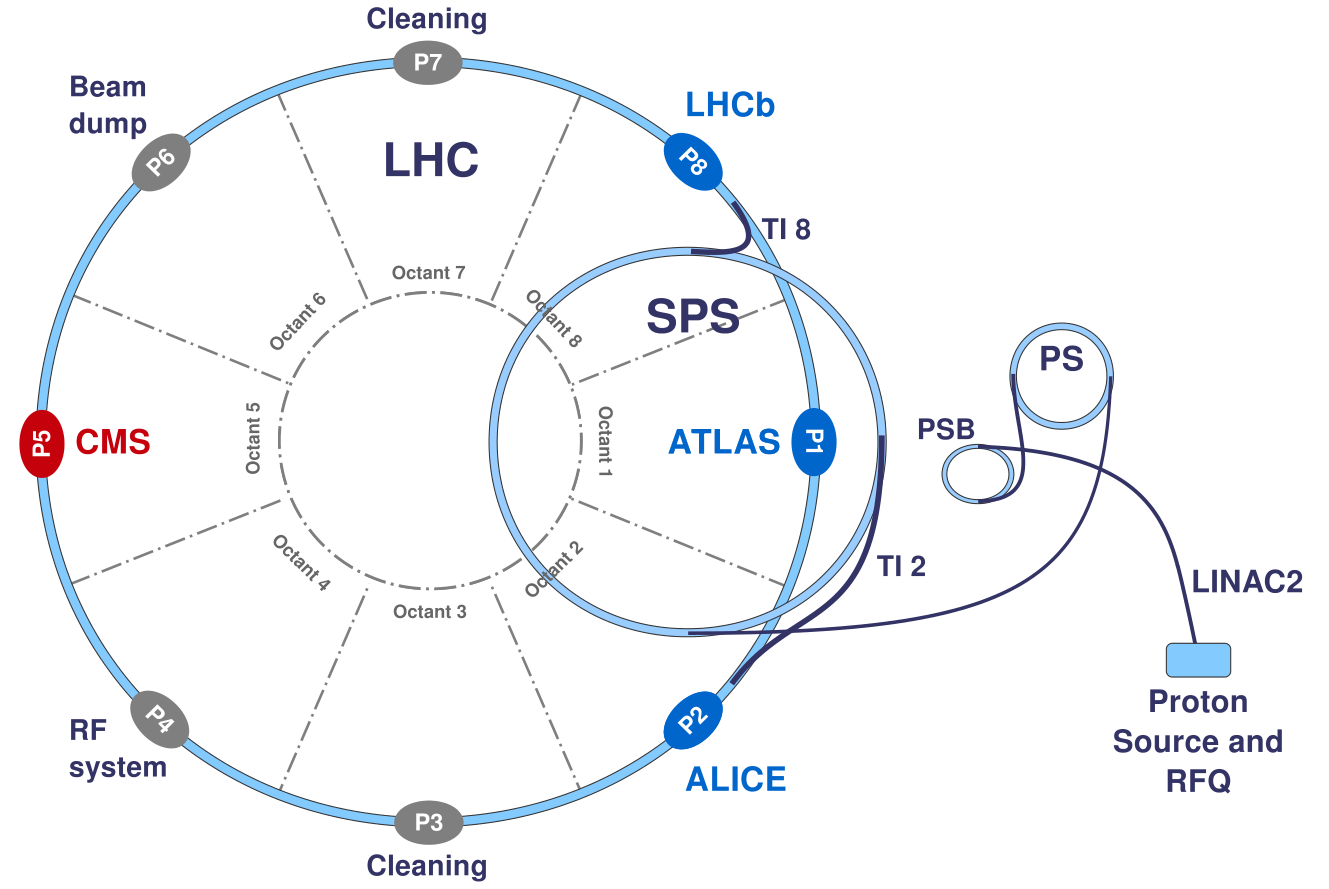
\includegraphics[height=0.4\textwidth]{images/lhc_aufbau.png}
  \caption{Schematic representation of the CERN accelerator complex (not to scale)\cite{lhc_aufbau}.}
  \label{fig:lhc_aufbau}
\end{figure}

After the second run from 2015 to 2018 followed the Long Shutdown 2 (LS2) until 2021 in order to upgrade the accelerator. The goal is to increase the luminosity by a factor of 10 by
implementing High Luminosity Large Hadron Collider (HL-LHC) in the Long Shutdown 3 (LS3), which is planned to be operational in 2026. Figure \ref{fig:lhc_plan} shows the timeline
of LHC programme.

\begin{figure}
  \centering
  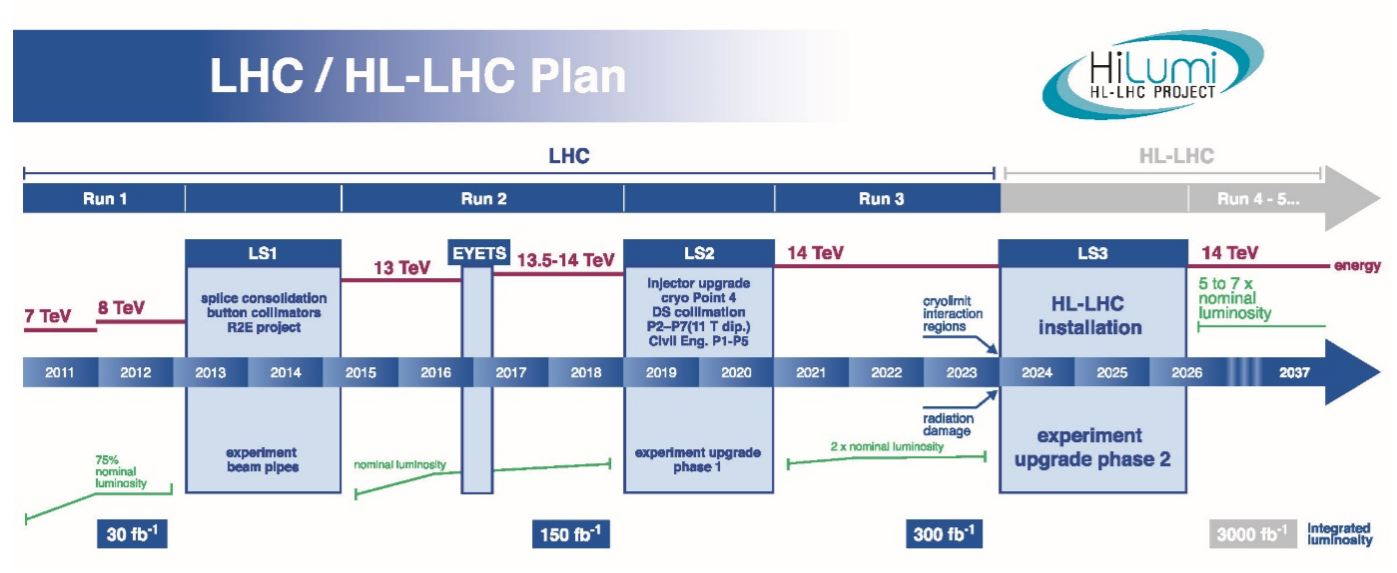
\includegraphics[height=0.4\textwidth]{images/lhc_plan.png}
  \caption{Timeline of the operational phases and Shutdowns of the LHC. The energy of accelerated protons in each phase is shown in red and the luminosity in green \cite{lhc_plan}.}
  \label{fig:lhc_plan}
\end{figure}

\section{The ATLAS detector}
The ATLAS detector is the largest general-purpose detector with a length of $\SI{46}{\meter}$ and a diameter of $\SI{25}{\meter}$.
It was designed to be a cylindric $4\pi$ detector, covering up most of the solid angle to detect particles flying in all directions.
Both ATLAS and CMS detected the Higgs Boson in 2012 and thus prove the existence of the last missing particle of the standard model.
Further goals of the detector is to search for beyond the standard model physics in the high energy domain, where current theories possibly break down.
Top quarks, which were produced at the LHC in large amount of quantities for the first time, can be studied more precisely with the help of the ATLAS detector.

The entire detector is made out of four different layers of detector systems, the Inner Detector, the electromagnetic and hadronic calorimeters
and the muon spectrometer. Only a couple of centimeter away from the interaction point lies the Inner Detector with its purpose to track the produced charged particles.
It is made of three subsequent components, with the innermost layer called the Pixel Detector and consists of three layers of silicon pixel detectors. The middle constituent
is the Semiconductor Tracker (SRT) with a similar purpose. Here, four layers of silicon stripe detectors are used for detection, while they have a lower spatial resolution, a larger
area can be covered with them more efficiently. The Transition Radiation Tracker (TRT) is the outermost component and uses straw detectors for tracking as well as materials with
different refractive index inbetween the straws. Relativistic particles will produce transition radiation by traversing these materials, which enables particle
identification, especially for light charged particles.
A magnetic solenoid surrounding the Inner Detector produces a $\SI{2}{\tesla}$ magnetic field to curve the trajectories of charged particles in order to determine their
momentum. \\
The electromagnetic calorimeter is positioned outside the magnetic field and aims at absorbing electrons, positrons and photon induced
electromagnetic showers in order to measure the energy of the initial particle. Lead and stainless steel serve as the energy absorbing material and liquid argon as the
sampling material. Hadrons tend to traverse the electromagnetic calorimeter without losing all their energy, which is the reason the hadronic calorimeter comes after.
It uses steel as sampling material and scintillating tiles to measure the energy. \\
Because muons easily pass both calorimeters, the outermost detector system is the muon spectrometer consisting of silicon detectors to track the muons and three toroidal magnets
building up a magnetic field for momentum measurement. Figure \ref{fig:atlas} ilustrates the ATLAS detector with its components.

\begin{figure}
  \centering
  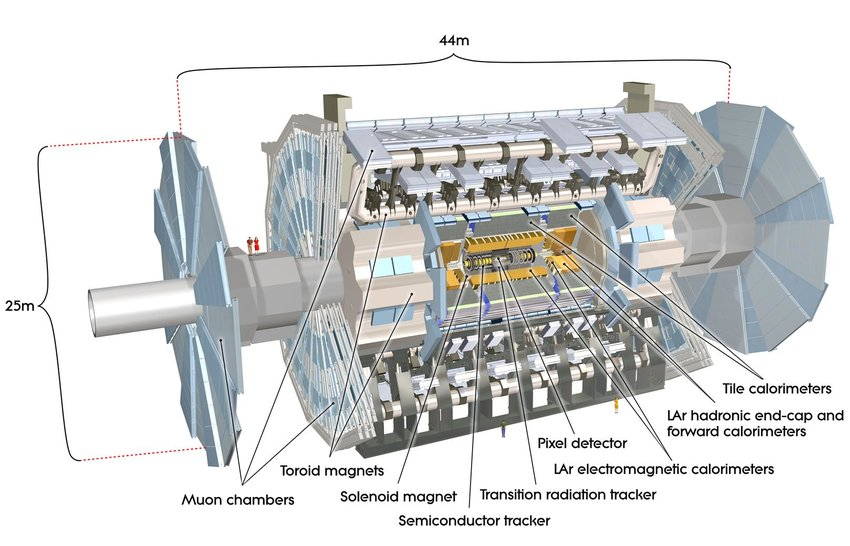
\includegraphics[height=0.5\textwidth]{images/atlas.png}
  \caption{Illustration of the ATLAS detector and its subsequent components. Two Humans are depicted at the bottom for a size comparison \cite{atlas}.}
  \label{fig:atlas}
\end{figure}

During the Long Shutdown 3 of the LHC, the ATLAS Inner Tracker (ITk) upgrade is planned to be installed. Its goal is to perform as good or better as the current detector, while
withstanding the harsher environment of the HL-LHC.

\chapter{Testbeam}
Studying the properties of sensor modules is crucial for an optimal performance of particle detectors. The new pixel modules used for the ATLAS ITk upgrade have to be thoroughly
tested in terms of efficiency and radiation hardness in order to fulfill the necessary requirements for their installment.
In order to evaluate the sensors performance they are irradiated in testbeam experiments similar to the conditions in the LHC.
These beam test measurements are performed mainly in two testbeam facilities, being located at Cern and Deutsches Elektronen Synchrotron (DESY). Sensors that are planned to be
installed in the ATLAS ITk are tested at DESY during the LS2.

\section{DESY Testbeam}
DESY is a national research center located at Hamburg. It operates the electron synchrotron DESY II since 1987 initially to accelerate electrons before injecting them into
HERA, the largest synchrotron at DESY. After the shut down of HERA in 2007, DESY II is now used for testbeam measurements. It produces an electron beam with energies upto
$\SI{7}{\GeV}$, which collides with a carbon fiber target creating bremsstrahlung in the process. The photons are extracted and collide with a secondary target
converting them to electron positron pairs. A dipole magnet behind the target creates a homogenous magnetic field to filter out unwanted energies and particles. This process
is shown schematically in figure \ref{fig:testbeam}.

\begin{figure}
  \centering
  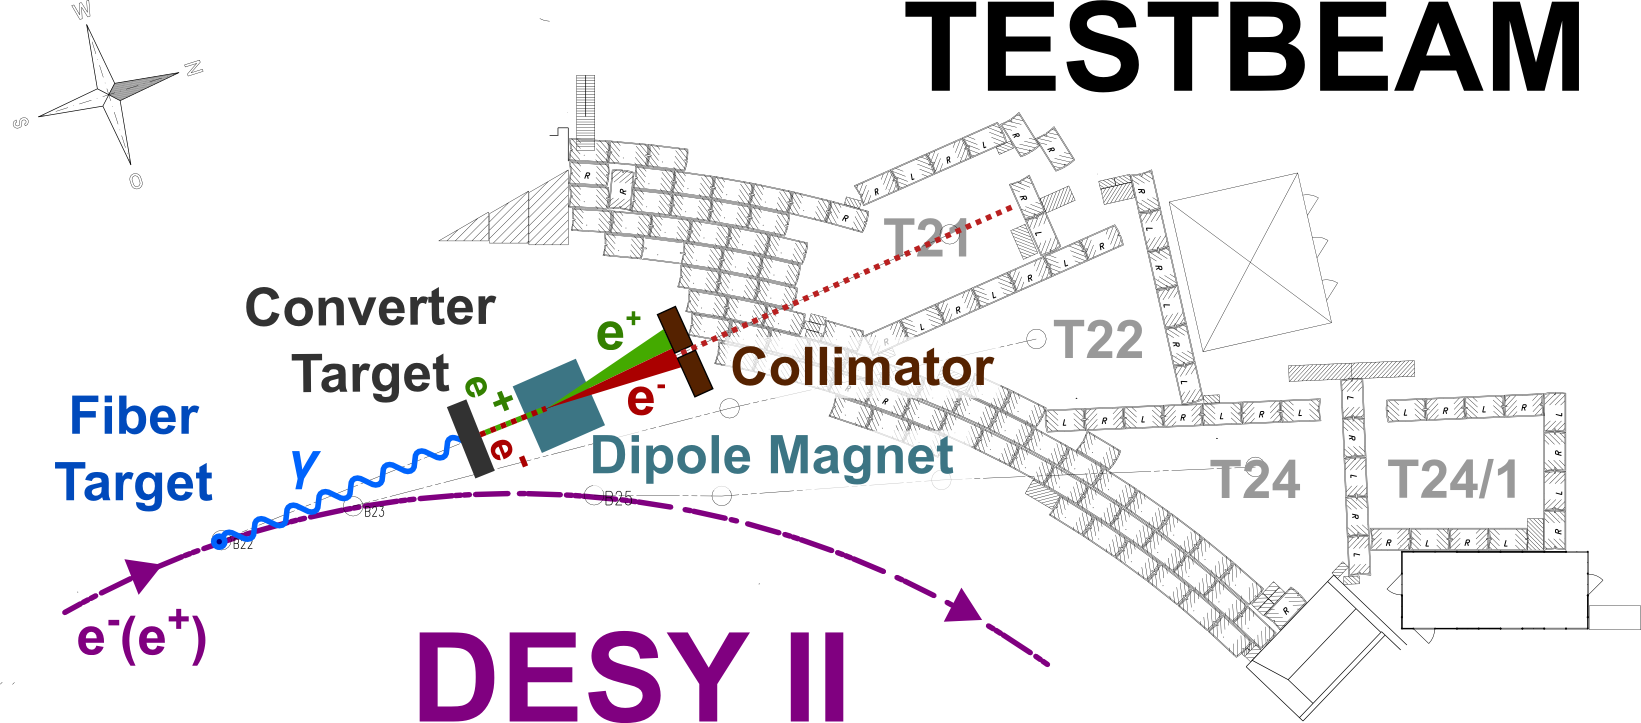
\includegraphics[height=0.4\textwidth]{images/desy.png}
  \caption{Depiction of the beam generation in testbeam experiments going through the beam line TB21 \cite{testbeam}.}
  \label{fig:testbeam}
\end{figure}

The permantly installed EUDET-type Pixel Beam telescopes DATURA and DURANTA are located behind the beam lines TB21 and TB22 and enable the tracking of the particles
produced by DESY II. Both telescopes consist of six Mimosa26 monolithic active pixel sensors with %a pixel pitch of $\SI{18.4}{\micro\meter} \times \SI{18.4}{\micro\meter}$.
three sensors each incorporated into one arm of the telescope and the DUT's being placed inbetween. A polystyrene box filled with dry ice is used to cool the DUT's to
avoid annealing and other unwanted effects due to heat. For time references during the measurements, an FE-I4 sensor is placed behind the telescope with a
time resolution of $\SI{25}{\nano\second}$ The sensors contain $336 \times 80$ pixels with a
$\SI{50}{\micro\meter} \times \SI{250}{\micro\meter}$ pixel pitch. Figure \ref{fig:telescope} shows the telescope setup of DATURA.

%\begin{figure}
%  \centering
%  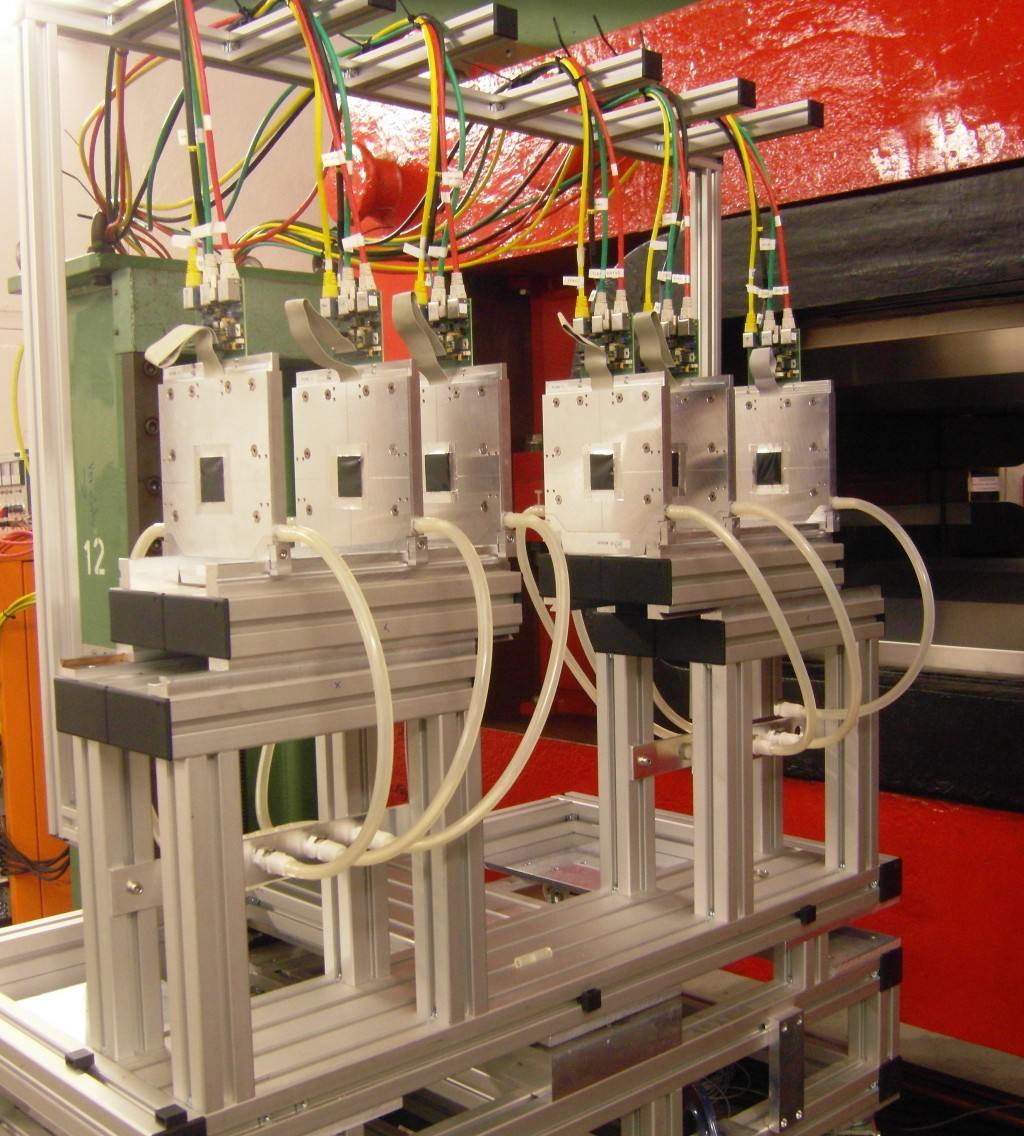
\includegraphics[height=0.4\textwidth]{images/telescope.jpg}
%  \caption{Shown is the Beam telescope DATURA consisting of six Mimosa26 sensors placed in the jigs. The tubes connected to the sensors transport water to
%  cool the sensors \cite{telescope}.}
%  \label{fig:telescope}
%\end{figure}

\begin{figure}
  %\centering
  \begin{subfigure}{0.48\textwidth}
      \centering
      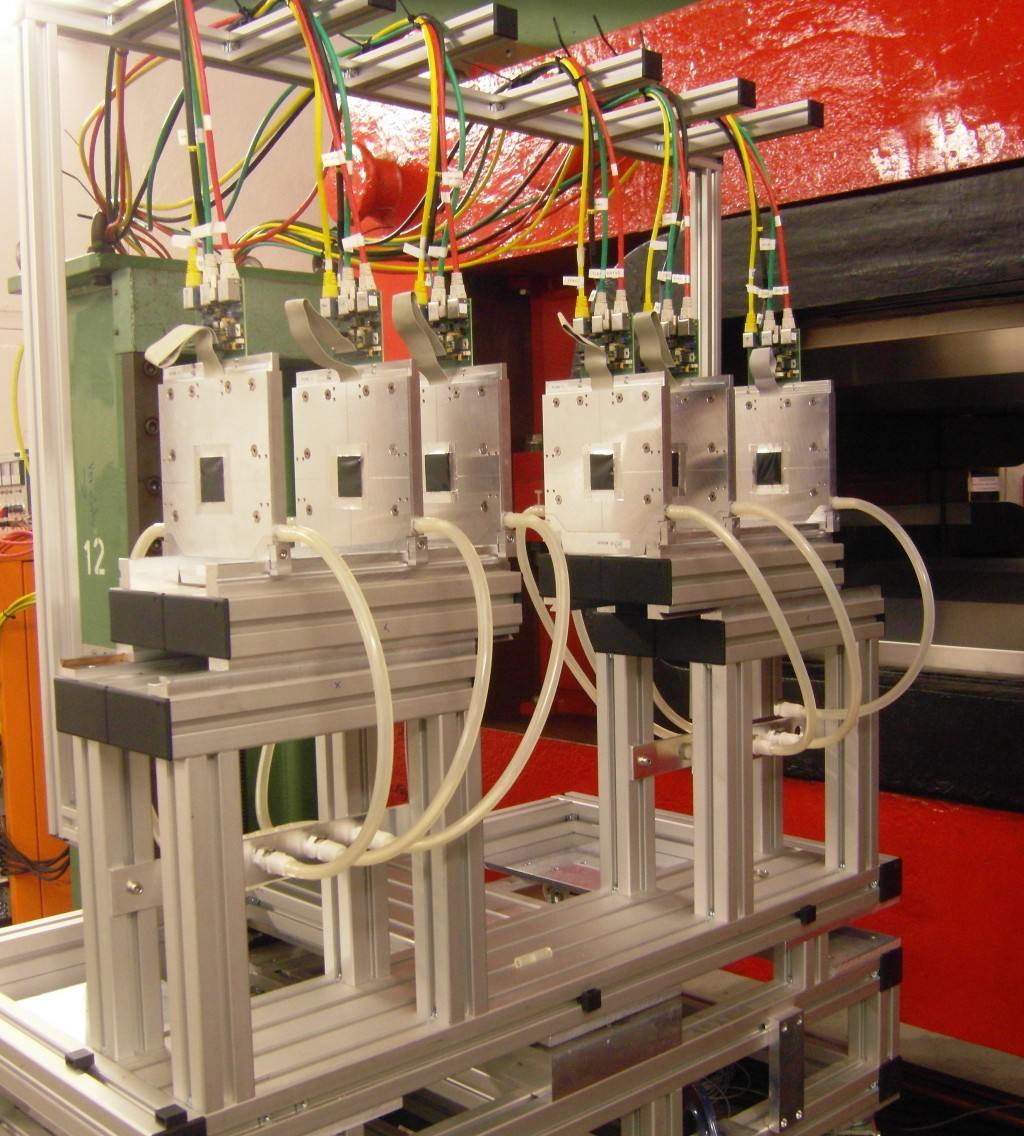
\includegraphics[height=0.82\textwidth]{images/telescope.jpg}
  \end{subfigure}
  \begin{subfigure}{0.48\textwidth}
      %\centering
      \hspace{-1cm}
      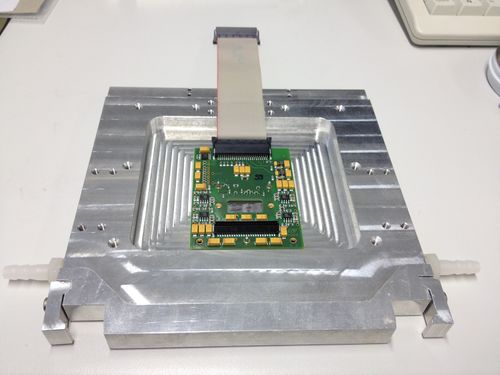
\includegraphics[height=0.82\textwidth]{images/mimosa.jpg}
  \end{subfigure}
  \caption{Shown on the left is the Beam telescope DATURA consisting of six Mimosa26 sensors placed in the jigs. The tubes connected to the sensors transport water to
  cool the sensors \cite{telescope}. Shown on the right is the Mimosa26 board inside the aluminium housing \cite{mimosa}. }
  \label{fig:telescope}
\end{figure}

Mimosa26 are fabricated in a standard $\SI{0.35}{\micro\meter}$ CMOS process with a fast binary read out
%size of $\SI{13.7}{\milli\meter} \times \SI{21.5}{\milli\meter}$.
Signals are measured with a time resolution of $\SI{230}{\micro\second}$ with each measurement in a read out cycle belonging to the same event.
They contain $576 \times 1152$ pixels with a pixel pitch of $\SI{18.4}{\micro\meter} \times \SI{18.4}{\micro\meter}$
and a thickness of $\SI{50}{\micro\meter}$.

The generic data aquisition framework EUDAQ records the data produced in testbeam experiments. Its centrally handles the data flow and synchronises data stream to enable
the integration of different independent devices under test. An exemplary setup of a beam telescope with EUDAQ is shown in figure \ref{fig:eudaq_bild}.
More information in \cite{eudaq}.

\begin{figure}
  \centering
  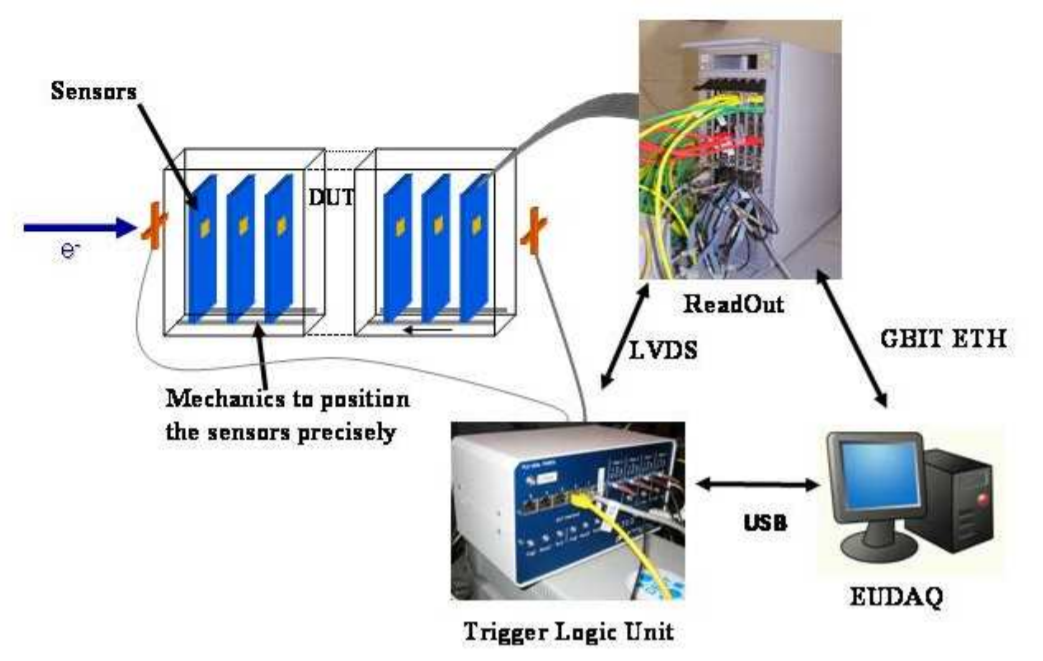
\includegraphics[height=0.4\textwidth]{images/eudaq.png}
  \caption{Necessary components for an analogue telescope \cite{eudaq_bild}.}
  \label{fig:eudaq_bild}
\end{figure}

\chapter{Track reconstruction}
The hit information of the sensor planes can be used to reconstruct the initial particles track. To properly reconstruct the tracks, multiple steps have to
be performed. For that reason entire frameworks were created to allow for a versatile and accurate track reconstruction to be possible. Two of the most
developed reconstruction softwares were used in this thesis and are explained in the following.

\section{The track reconstruction framework EUTelescope}
In order to do that the sotware EUTelescope was developed and
primarily used since 2007. It uses the Modular Analysis and Reconstruction for the Linear Collider (MARLIN) framework, which is part of the
International Collider Software package (ILCSoft). Each step in the reconstruction depends on MARLIN processors, which read in data, modifies and outputs new data to be
taken by the next processors. The individual steps in the reconstruction will call on certain processors specified for its task resulting in a
modular structure.

Information about the telescope geometry is stored in  Geometry API for Reconstruction (GEAR) files. This includes the position and rotation
of the sensors as well as their pixel layouts. Further parameters like radiation hardness, magnetic field and general properties of the used sensors have to be
specified to ensure proper track reconstruction.

General parameters and parameters in individual reconstruction steps are specified in the configuration file. This includes the import of the raw data and the
geometry file, the applied reconstruction steps and the definition of the cuts. \\
The steering files define the processors used in each reconstruction step and in which order they are executed.
A complete track reconstruction with EUTelescope contains the converter, the clustering, the hitmaker, the alignment and the track fitting in this respective order.
The overall track reconstruction of EUTelescope is shown in figure \ref{fig:track_reco} with the most important steps explained in the following.

\begin{figure}
  \centering
  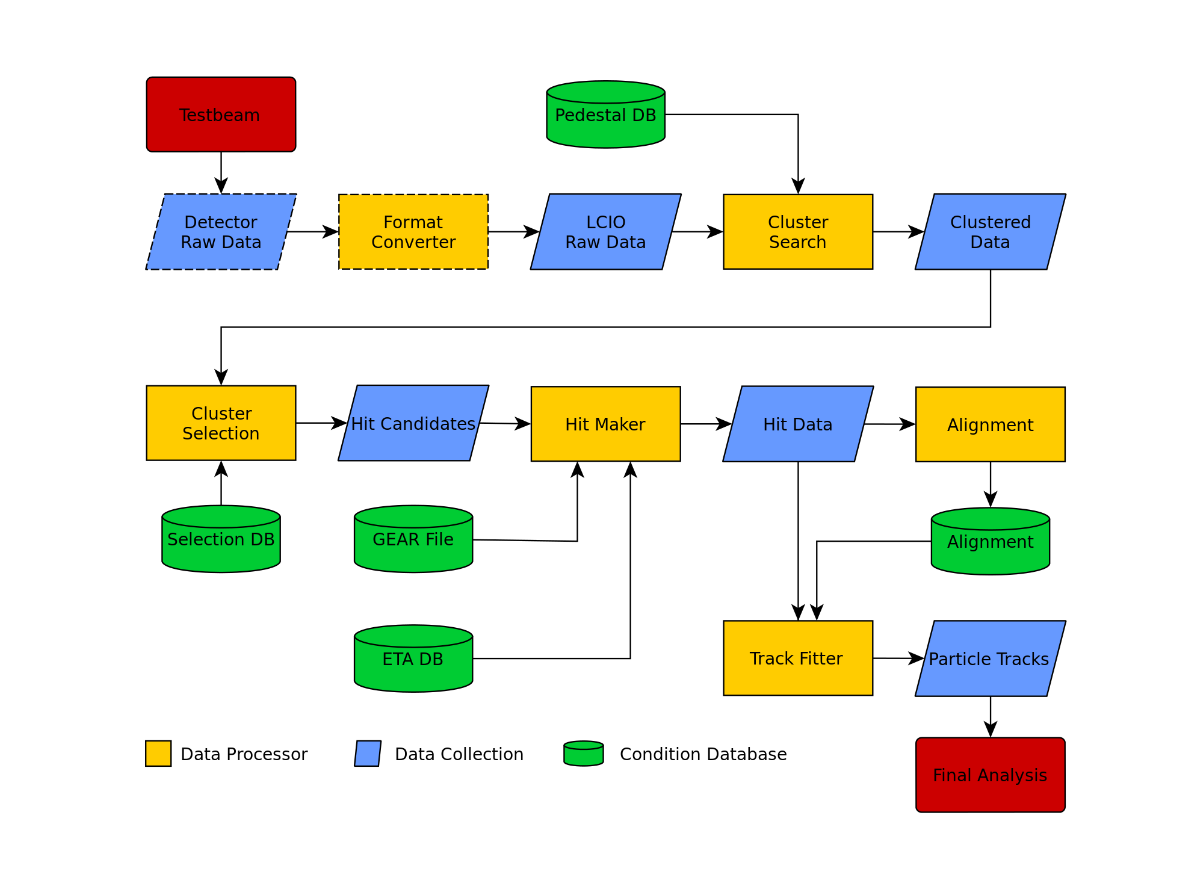
\includegraphics[height=0.6\textwidth]{images/track_reco.png}
  \caption{The overall track reconstruction of EUTelescope including the MARLIN processors and files. \cite{track_reco}.}
  \label{fig:track_reco}
\end{figure}

First, the raw data has to be converted to the lcio format for subsequent MARLIN processors. In addition, the module detects noisy pixels by analysing the
hit rate of the pixels and dividing them by the sum of measured events. The resulting firing frequency can be limited by user defined cuts, thus removing entries
from noise considered pixels from the lcio file.

In the clustering process, hit information on a sensor plane generated by the same particle will be clustered. Cluster with more than one pixel occur due
particles traversing through multiple pixels or charge sharing. Pixels will be grouped together based on their distance.
Regulation of the clustering process is then possible with cuts on the pixel distances.

The hitmaker step determines the particles hit position, the cluster center, of each cluster. For one pixel cluster, the cluster center is equal to the middle of
te pixel. Cluster centers of clusters with more than one pixel are calculated with a charge weighted center of gravity algorithm. This means, that
the deposited charge of each pixel is taken into account to derive the particles position. The cluster centers are transformed to the global coordinate
system of the telescope to function as the hit position for the track reconstruction. Global hit information on the sensors of particle tracks is assumed to be correlated with only
a small spread of the beam angle, which makes an initial guess of the telescope alignment, the prealignment, possible. With the prealignment it is possible
to correct larger misplacements of the sensors.

To compensate possible misaligment of sensors in the telescope, the alignment processor tries to optimise the setup. Cluster information from the hitmaker
are used to fit tracks through the planes and correct deviations by rotating and shifting the sensors. After the alignment process is finished a new gear file is produced, which
is then used for further reconstruction steps. Usually, several iterations of the alignment process occur to determine the optimal positions of the sensor planes
in the telescope.
There are two major processors for the alignment step, which implement different track fitting algorithms.
The DAF processor is based on a Kalman filter and was specifically designed for high noise environments. It uses the inbuild combinatorics filter, which fits
straight line tracks through all combinations of clusters allowed by the specified cuts and only keeps the ones with a minimum $\chi^2$. Here, the $\chi^2$ parameter
describes the goodness of the fit and is defined as:
\begin{align}
  \chi^2 = \sum_i (r_x/\sigma_x)^2 + (r_y/\sigma_y)^2
\end{align}

The parameters $r_x$ and $r_y$ refer to the residuals on each sensor in X and Y direction, which describe the distance of the cluster center used for the track fit and the
position of the track on a plane. All residuals are weighted with their spatial resolution $\sigma_x$ and $\sigma_y$ for each sensor. \\
The second fitter uses the General Broken Line (GBL) algorithm with a separate patter recognition processor for track fitting. Kinematics of
beam particles are used to predict hits belonging to a track. In the track finding process, two straight lines are fitted through the upstream and
downstream sensors, whenever the user defined cuts on the slope allow it. The two straight lines are extrapolated to the centre of the telescope, where
they form the overall track depending on their distance to each other and the corresponding user defined cut.\\
Fitted tracks used for the alignment are handled by the Millipede II processor. It performs least squares minimisation for a particular set of problems, which
have an interest of global parameters over local parameters in common. Thus, Millepede II is able to align the planes with any applied track model.

After the alignment is finished the tracks are fully reconstructed with either the DAF or the GBL fitter. Optionally, DUT's can be included in the fitting
process, however it is usually avoided to keep the residuals of the DUT unbiased. In the scope of this thesis, the GBL processor is used for the
alignment and fitting step. To reconstruct a track, the fitGBL processor uses GBL points, which carry a series of attributes. These points can either be a
hit or an other point of interest on the trajectory. Figure \ref{fig:gbl} depicts an exemplary reconstructed track with the fitGBL processor.

\begin{figure}
  \centering
  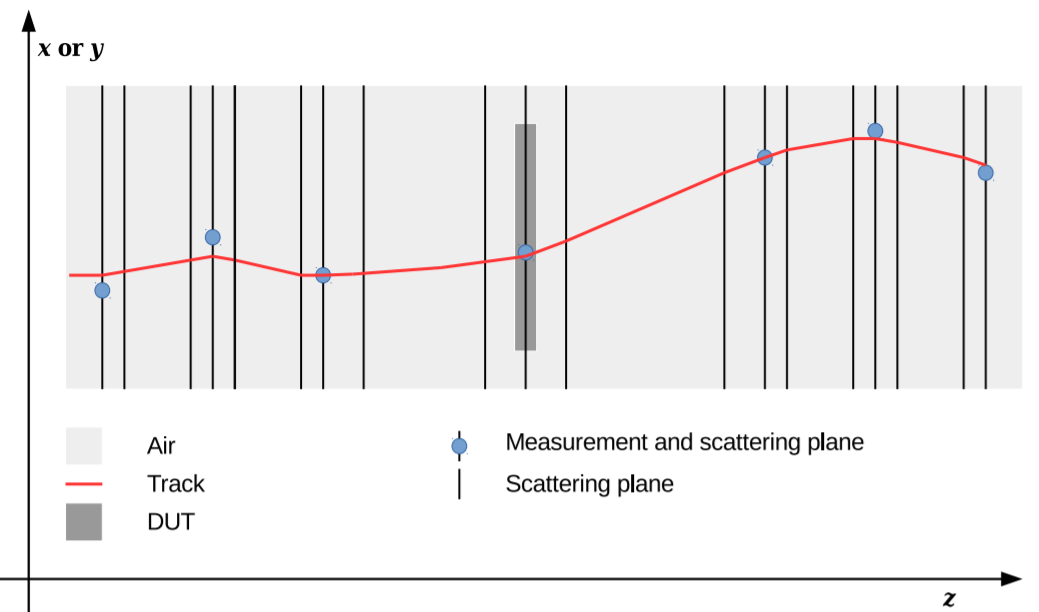
\includegraphics[height=0.5\textwidth]{images/gbl.png}
  \caption{Track reconstruction with the fitGBL processor. Scatterering points are connected with a straight line. \cite{gbl}.}
  \label{fig:gbl}
\end{figure}



\section{The track reconstruction framework Corryvreckan}
Corryvreckan is a fast and lightweight track reconstruction framework released in 2017 and is the most developed alternative to the EUTelescope software.
Since the development and support of the EUTelescope discontinued, Corryvreckan is planned to supersede the former as the primarily used track
reconstruction software. Its main advantage is the minimal amount of external dependencies connected to the software and the more user friendly usage of
it.
Corryvreckans structure is based on the modular concept of the simulation software Allpix$^2$, making the software flexible and ensures to meet the requirements for track reconstruction in
complex environments. Global parameters and modules used for the track reconstruction are specified in the configuration file, which starts the event loop upon
executing. Data and the geometry of the setup are both imported into the configuration file as well. A reference sensor has to be specified in the geometry folder
for which the rest of the telescope is aligned with.

During event processing, information taken and produced by the modules are temporarily stored on the clipboard, serving as the infratructure for temporary
storing information. %the event, the
%temporary data storage and the persistent storage. The event is the central element storing information about the currently processed data.
The necessary steps in the track reconstruction chain of the software are similar to ones taken in EUTelescope and are explained in the following.

To load the taken data into Corryvreckan a certain eventloader module is used depending on the data format. The order of Eventloader modules
is important as the first module loaded will define the event on the clipboard either through trigger numbers or a time window. Measurements stored with EUDAQ are loaded with the
EventloaderEUDAQ module, which requires the EUDAQ library as an external dependency. Altneratively to the eventloader modules, data in root format can also be imported
with the FileReader module, which is mainly used for simulated data or data written out with the FileWriter module.

The clustering process can be either done with the Clustering4D or the ClusteringSpatial module, with the former being the standard clustering module taking hit timestamps
into account. Spatial and timing cuts can be defined by the user either through absolute values or relative factors multiplied by the sensors spatial and time resolution. Both
center of gravity or arithmetic mean calculations for the cluster centre can be chosen.


While not mandatory for the overall track reconstruction chain, a correlation module can be applied to create several correlation plots, taking the hit information
from the clipboard to plot their location against the ones of the reference sensor. These plots can then be used to identify major translational and
rotational misalignments of sensors.  Either an abolute or relative time cut can be specified for clusters on a sensor to be considered in respect to
the reference sensor.

The Prealignment module accounts for major tranlational misplacements of sensors and performs translational shifts along the X and Y axis of up to several millimeter to ensure a proper alignment later on, as higher misaligmnents might cause the main alignment process to not converge correctly.
To calculate the applied shifts, the mean of the 1D correlation
histograms of each detector is used. A  relative or absolute time cut can be specified.

Reconstructing tracks from cluster centres can then be accomplished with the Tracking4D or Trackingspatial module. Similar to the clustering modules, only the former
takes timestamp information into account and is therfore the standard track reconstruction module. For the track finding process, clusters on the first plane are
related to clusters close in time on subsequent planes using straight lines.
The Tracking4D module has two possible track models, straight lines as default setting and general
broken lines, for fitting. General broken lines account for multiple coulomb scattering and considers scattering at every sensor plane as well as the surrounding air.
Absolute and relative spatial and time cuts can be specified, as well as the minimum number
of clusters necessary to fit a track. The DUT can be included reconstruction process, though this is avoided in this thesis to keep the residuals of DUT's unbiased.


To align the telescope, the AlignmentTrackChi2 module is used. It performs rotational and translational telescope
alignment according to minimise the $\chi^2$ value by iterating through all planes and refitting the tracks after alignment. Cuts on the $\chi^2$ value can be
applied to only keep high quality tracks. Furthermore, the number of iterations of the alignment method can be specified.

After successful alignment, the DUTAssociation module uses the cluster information of the DUT to establish an association with reconstructed tracks. Again, absolute
and relative spatial and time cuts can be specified. It can also be chosen wether the nearest pixel of the cluster or the cluster centre is compared with the track.
With the associated tracks the DUT's are aligned in the AlignmentDUTResidual module with the same adjustable parameters as the AlignmentTrackChi2 module.
The AnalysisDUT module then creates the residual plots of the dut with an optinal cut on the $\chi^2$ value. Sensor efficiencies of the DUT's are determined with the
AnalysisEfficiency module by comparing cluster positions with the interpolated tracks.


Figure \ref{fig:corry_track_reco} depicts
the different modules used for a general track reconstruction. The entire Corryvreckan framework is documented in detail for further information \cite{corry_manual}.

\begin{figure}
  \centering
  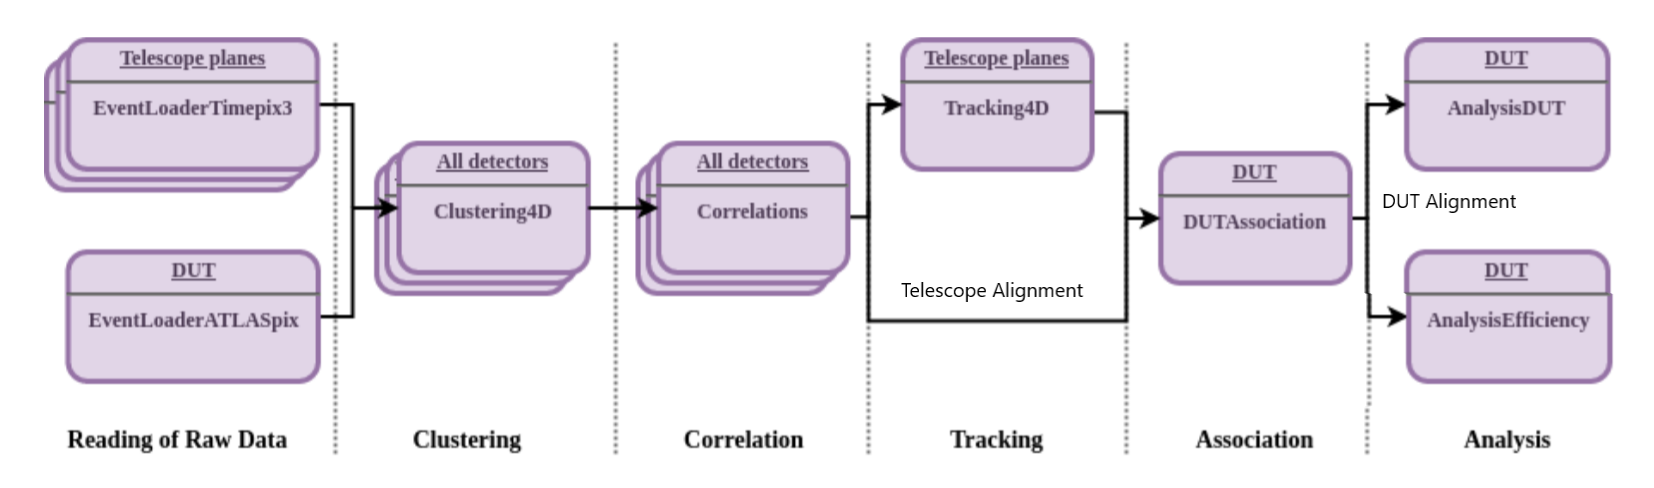
\includegraphics[height=0.3\textwidth]{images/corry.png}
  \caption{Overall track reconstruction chain with the standard clustering and tracking module. \cite{corry_track_reco}.}
  \label{fig:corry_track_reco}
\end{figure}


\chapter{The simulation software Allpix$^2$}
Allpix$^2$ is a generic simulation framework developed at CERN to simulate the performance of silicon detectors and was released in 2017. It builds upon the
Geant4 \cite{geant4} package to perform tasks in the simulation chain. The main tasks of Allpix$^2$ is the simulation of energy depostions of particles
in the sensors, the propagation of charge carriers in the sensor material and the digitization of the signal. It has a modular
structure to ensure an easy handling, while still allowing for complex detector simulations. Instantiation and processing of the modules is done by the core of the framework,
which contains five subsystems. This includes the configuration containing the configuration manager, which grants access to the configuration file, the
module subsystem, which loads and executes the modules and the geometry subsystem, which provides the information of the telescope setup. Objects are transferred
from one module to another with the messenger subsystem.
Figure \ref{fig:allpix} depicts the overall structure of Allpix$^2$.

\begin{figure}
  \centering
  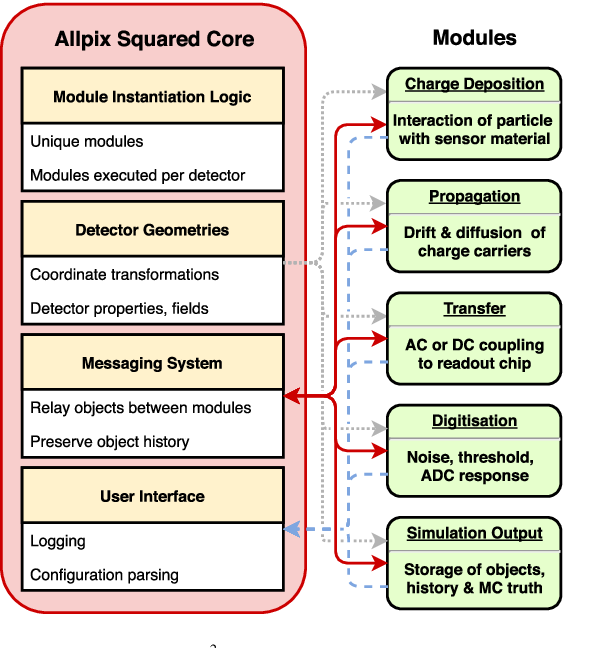
\includegraphics[height=0.5\textwidth]{images/allpix.png}
  \caption{Schematic representation of the overall Allpix$^2$ structure. \cite{fig_allpix}.}
  \label{fig:allpix}
\end{figure}

The telescope geometry has to be specified in a geometry file, which includes all sensors and their pixel matrix as well as their spatial and time resolution. Additionally,
the position and orientation have to be stated. Optionally, uncertainties on the position and orientation can be set to account for misalignment in real telescope setups.
In the configuration file, the geometry is imported as well as the modules for the simulation in order of execution, which
will be explained in the following.

The world frame of the simulation is created with the GeometryBuilderGeant4 module. The world material can be either air or vacuum with a configurable world margin percentage.
Afterwards all detectors from the internal detector models and passive material models are created according to the specifications in the geometry file.

Charge carriers are deposited in the active volume with the DepositionGeant4 module, which initializes the simulation of particles. The shape of the source beam, as well
as the type of particle and its energy can be specified. Further parameters are the width of the beam, its angular distribution based on a gaussian distribution and the energy
uncertainty of the simulated particles. All particles created at the same time define an event. The number of generated electron hole pairs is calculated with the
mean pair creation energy and is subject to fluctuations, which are defined by the fano factor.

An electric field is added to the sensors with the ElectricFieldReader module. By default all sensors are targeted by the module, though specific sensors can be stated.
There are three types of electric field models available, constant electric fields, linear electric fields and external simulated electric fields, with only
linear electric fiels being used in the scope of this thesis. The constant slope of linear electirc fields are defined by the bias voltage and the
depletion voltage of the sensor. Optionally, the depletion depth instead of the depletion voltage can be specified.

Either with the ProjectionPropagation or the GenericPropagation module the transport of charge carriers through the sensitive material are simulated.
The first module projects electrons or hole onto the surface and performs a randomized diffusion based on a two dimensional gaussian distribution around
the projection. Using an approximation of the drift time makes it possible to determine the diffusion width under the assumption of a linear electric field. This
module save computing time at the cost of accuracy. \\
The GenericPropagation module consists of a combined simulation of diffusion and drift calculated with a Runge-Kutter-Fehlberg method.
It is compatible with any electric field model and can simulate both electrons and holes
at the same time making the module
more accurate at the cost of computing time. The integration time can be specified by the user to determine the time of the propagation process. \\
In both modules, charge carriers are combined to sets and propagated together with no interaction between them. The set size of charge carriers can be specified by the user,
making it possible to control the accuracy and computing time of the simulation. For diffusion simulations it is necessary to specifiy the temperature of the sensor material
to calculate the diffusion constant.

Sets of charges are combined on the sensor pixels with the SimpleTransfer module and are prepared  to be processed by the front-end chips. The
propagated charges are mapped directly to the nearest pixel, while charge carriers that are outside the pixel grid or too far away from the implants are ignored.

Collected charges are then translated into digitised signals proportional to the input charge by the DefaultDigitizer module. Additionally, gaussian noise constributions
from the readout electronics can be simulated and a signal threshold can be defined. The output signal is given in units of the electron charge per default, but
can also be given in bits by simulating a QDC converter. Optionally, a gain factor and gain smearing can be set.

Simulated events and the produced plots of the different modules are stored in a root file. With the ROOTObjectWriter module further information like propagated charge,
deposited charge, Monte Carlo (MC) particle information and pixel hit information are stored in an additional ROOT file. Allpix$^2$ also enables the storing of
data in formats compatible with the EUTelescope and Corryvreckan software with the LCIOWriter module and the CorryvreckanWriter module respectively. Both modules possess parameters, which
determine what information of the Allpix$^2$ simulation is written into the ROOT files.


\chapter{Radiation therapy}
Radiation therapies are medical treatments using ionizing radiation mainly to kill cancer cells in patients. The ionizing particles interact with the
cancer cells to damage their DNA causing cellular death. These treatments focus on cancer that is localized to one area inside the body. \\
The type of particle used in radiation therapy is crucial to the overall treatment due to the different interaction of particles with the human body.
Photons, specifically x-rays, are the most common particles being used for radiation therapy.
A newer alternative is the proton therapy, due to the different properties protons giving advantages over conventional x-ray therapy explained in the following section.

\section{Proton therapy}
The proton therapy is an external beam radiotherapy using a proton beam for irradiation. While proton therapy centres have only been used since 1889 the technological
advancement ensures the continual rise of hospitals offering proton therapy.
The proton therapy centres either use cyclotrons or synchrotron to accelerate the protons, with the former being compact and simple to operate and the latter being able
to produce protons of varying energies from $\SI{50}{\MeV}$ to $\SI{250}{\MeV}$.
Unlike photons, which tend to deposit their entire energy in a single ionisation process, protons undergo multiple coulomb scattering inside matter. The
energy loss of protons is inversely proportional to the sqaure of their velocity, which causes them to deposit most of their energy on the last millimeters of their path.
This beaviour is called the Bragg peak and is shown in figure \ref{fig:bragg}. Regulating the energy of the protons allows for precise control of the Bragg peak depth inside
the human body.

\begin{figure}
  \centering
  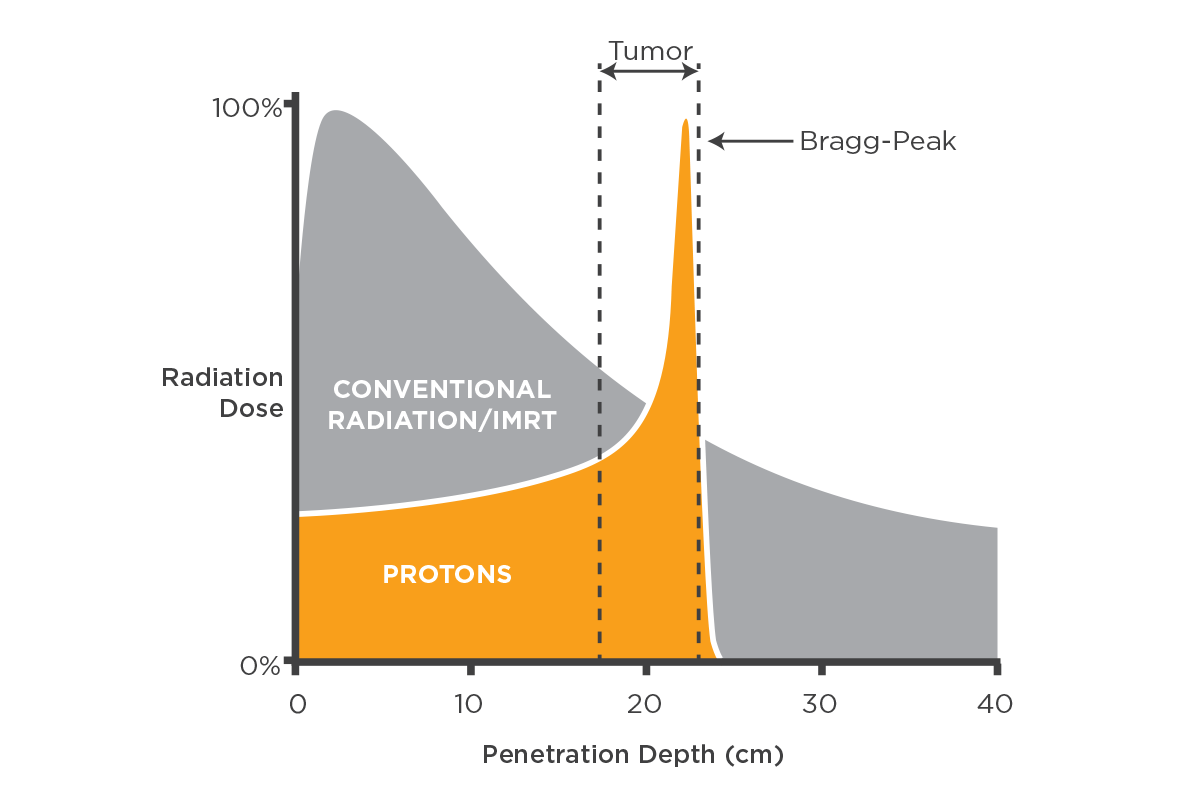
\includegraphics[height=0.6\textwidth]{images/bragg.png}
  \caption{Radiation dose of protons and x-rays as a function of the penetration depth. Protons deposit most of their energy in a localized spot, while
  x-rays deposit energy in a much borader region.}
  \label{fig:bragg}
\end{figure}
Due to this property, protons enable to irradiate tumors with greater precision than with
x-rays, as surrounding healthy tissue is less damaged, especially behind the tumor. Figure \ref{fig:risk} shows the irradiated areas of a brain for conventional and
proton therapy to emphasise their differences.

\begin{figure}
  \centering
  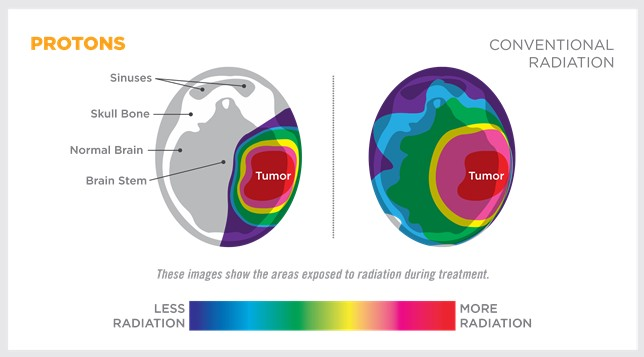
\includegraphics[height=0.5\textwidth]{images/risk.png}
  \caption{Radiated region for protons and x-rays to trea a brain tumor. The irradiation for proton therapy is far more precise and damages less healthy tissue than
  x-ray therapy.}
  \label{fig:risk}
\end{figure}


\section{Computed tomography} \label{sec:ct}
To irradiate a patient save and efficiently it is necessary to create an irradiation plan by identifying the tumor and the surrounding healthy tissue. In order to do so a computed
tomography (ct) scan is performed using a particle beam to create an image of the region encompassing the tumor. For x-ray therapy as well as proton therapy x-ray ct scans
are used primarily. \\
To create an image, the patient lies within a rotating x-ray tube, the gantry, which generates x-ray beams to irradiate the specific volume. The gantry also
includes a row of detectors measuring the photons after traversing the human body. Due to the fact that different tissue materials inside the body absorb a different
amount of light, a projection of the irradiated volume can be created. By rotating the x-ray tube, projections are created from many different angles around the patient.
Unlike in radiography, where two dimensional projections are produced, ct scan measurements are one dimensional absorption profiles. The sum of the profiles contain
the entire information of the inside structure, but can not be interpreted directly. Projections and the original three dimensional structure are connected through
the inverse radon transformation. An implementation of that algorithm is the filtered back projection:
\begin{align}
  f(x,y) = \int_0^{\pi} \left(\int_{-\infty}^{\infty} p_{\phi}(z') \cdot g(z - z') \mathrm{d}z'\right) \mathrm{d}\phi
\end{align}
Where $f(x,y)$ is the original image, $p_{\phi}(z)$ the projection in the direction of the angle $\phi$ and $g(z)$ a high-pass filter. However, the inverse
radon tranformation is an ill posed problem, which demands an irregular filter kernel g(z). To solve this problem in praxis, a fast convolution algorithm is used for the
filtered back projection. This means that the projection is multiplied with the high-pass filter in fourier space, where each frequency component is weighted proportional to their
absolute value. In the end, each one dimensional projection is stretched into two dimensions and rotated around the angle $-\phi$. The sum over all projections will yield the
final image.


\section{Proton computed tomogrophy}
Creating irradiation plans for proton therapy with x-ray ct images causes larger uncertainty due to the different stopping powers of the particles.
To compensate for the differences,a range uncertainty margin is applied to the prescribed range, which increases with greater travel distance through the body. This
method is shown in figure \ref{fig:paganetti}.

\begin{figure}
  \centering
  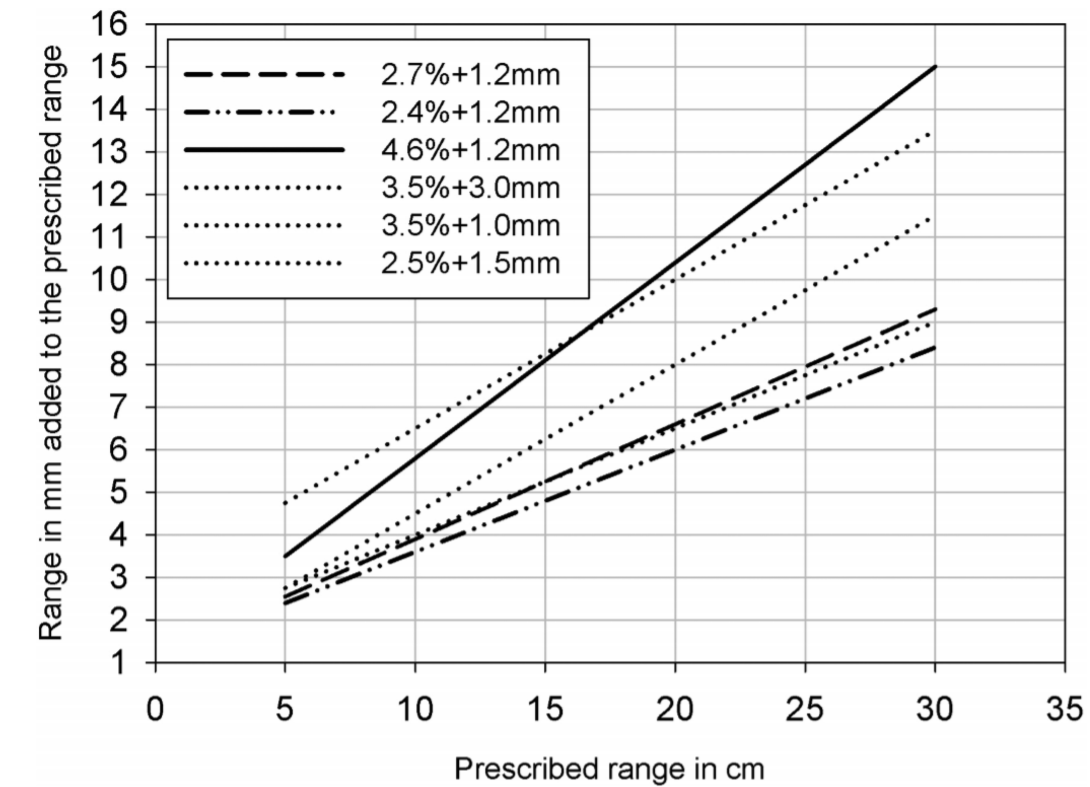
\includegraphics[height=0.6\textwidth]{images/prescription.png}
  \caption{Applied uncertainty margins at the Massachusetts General Hospital (3.5\,\% +
1mm), the MD Anderson Proton Therapy Center in Houston (3.5\,\% + 3mm), the Loma Linda
University Medical Center (3.5\,\% + 3mm), the Roberts Proton Therapy Center at the
University of Pennsylvania (3.5\,\% + 3mm), and the University of Florida Proton Therapy
Institute (2.5\,\% + 1.5mm), shown as dashed lines. Dashed-dotted and dashed line: Uncertainty margin for with and without the use of Monte Carlo dose calculation.
The solid-line describes the safety margin for complex geometries without Monte Carlo dose calculation \cite{paganetti}.}
  \label{fig:paganetti}
\end{figure}

Since the position of the protons energy deposition has to be determined as precise as possible to minimise damage dealt to healthy tissue, a computed tomogrophy scan using protons
is a promising alternative to conventional ct. Creating an image with proton ct is similar to conventional. A proton beam irradiates and deposits energy in the patient. The
protons remaining energy is then measured with a calorimeter system behind the patient to gain information about the composition of the tissue. A projection can be created,
if the protons tracks can be reconstructed. However, due to multiple coulomb scatterings of the protons inside the patient, the spatial resolution will decrease in comparison
to conventional ct. Numerous projections are created by varying the angle of the proton beam in respect to the target. The entire setup is schematically in figure \ref{fig:proton_ct}.

\begin{figure}
  \centering
  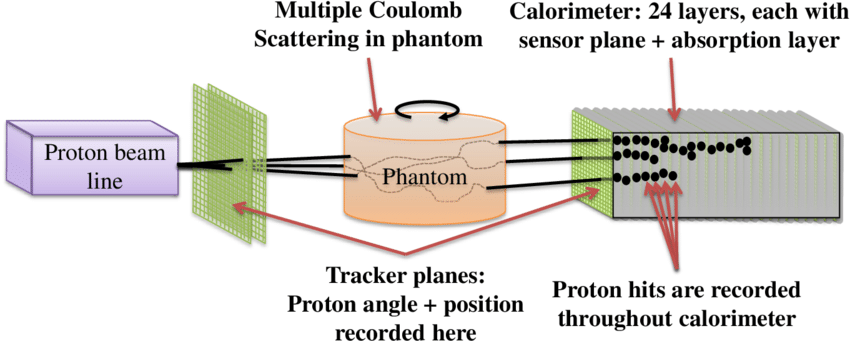
\includegraphics[height=0.4\textwidth]{images/proton_ct.png}
  \caption{Procedure of the proton computed tomogrophy. The tracker planes are used to reconstruct the proton tracks and the calorimeter to measure their remaining energy.
  The phantom is the placeholder of a patient \cite{proton_ct}.}
  \label{fig:proton_ct}
\end{figure}

The different projections can then be reconstructed to a complete image of the irradiated volume as explained in section \ref{sec:ct}.
